\chapter{Requirements}
\label{chap:requirements}

This chapter introduces the pulverization approach by explaining the terminologies and concepts that will be used in the rest of the thesis.
The main principles of pulverization are presented, followed by a description of the pulverization domain model supported by some relevant examples.
Next, the framework's requirements are reported and, finally, the chapter concludes with relevant scenarios that are worth using to test the use and
effectiveness of the framework.

\section{Pulverization domain model}
\label{sec:pulverization-domain-model}

Pulverization is an approach to conceive self-organization in distributed systems that facilitate deployment independence, i.e., the ability of an
application to run with no change on various deployments while retaining its original functional semantics.
The main idea is to organize the structure and the behaviour of a system in a way that the developer can focus on the logical model, abstracting from
the deployment details, scheduling and communication.
The logical model can be partitioned into a set of software components that can be deployed on the available infrastructure, while the application
logic will preserve the functional goals independently from the actual deployment.

To better formalize the terminology coming from the pulverization, the following \emph{ubiquitous language}~\cite{evans2004ddd} is proposed
in~\Cref{tab:ubiquitous-language}.
The main reasons for the use of this ubiquitous language are to avoid ambiguity and to ensure that the concepts are understood in the same way by
anyone who approaches the pulverization.

\begin{table}
	\begin{tabularx}{\textwidth}{l X}
		\toprule
		\textbf{Concept}          & \textbf{Definition}                                                                                             \\
		\midrule
		Sensors                   & Component that represents a set of logical \emph{sensors}                                                       \\
		Actuators                 & Component that represents a set of logical \emph{actuators}                                                     \\
		Behaviour                 & Component that models the device behaviour                                                                      \\
		Communication             & Component that handles the interaction with neighbours (other devices)                                          \\
		State                     & Component the holds the representation of the device's knowledge                                                \\
		Thin host                 & A device that has limited computational power and memory                                                        \\
		Thick host                & A device that has a powerful computational power and memory                                                     \\
		Logical device            & A logical representation of a device composed of several components which they can be deployed on the available
		infrastructure                                                                                                                              \\
		Logical neighbouring link & Defines a logical connection between two logical devices defining the network topology.
		The aforementioned structure can change over time.                                                                                          \\
		\bottomrule
	\end{tabularx}
	\caption{Pulverization Ubiquitous language.}
	\label{tab:ubiquitous-language}
\end{table}

\begin{figure}
	\centering
	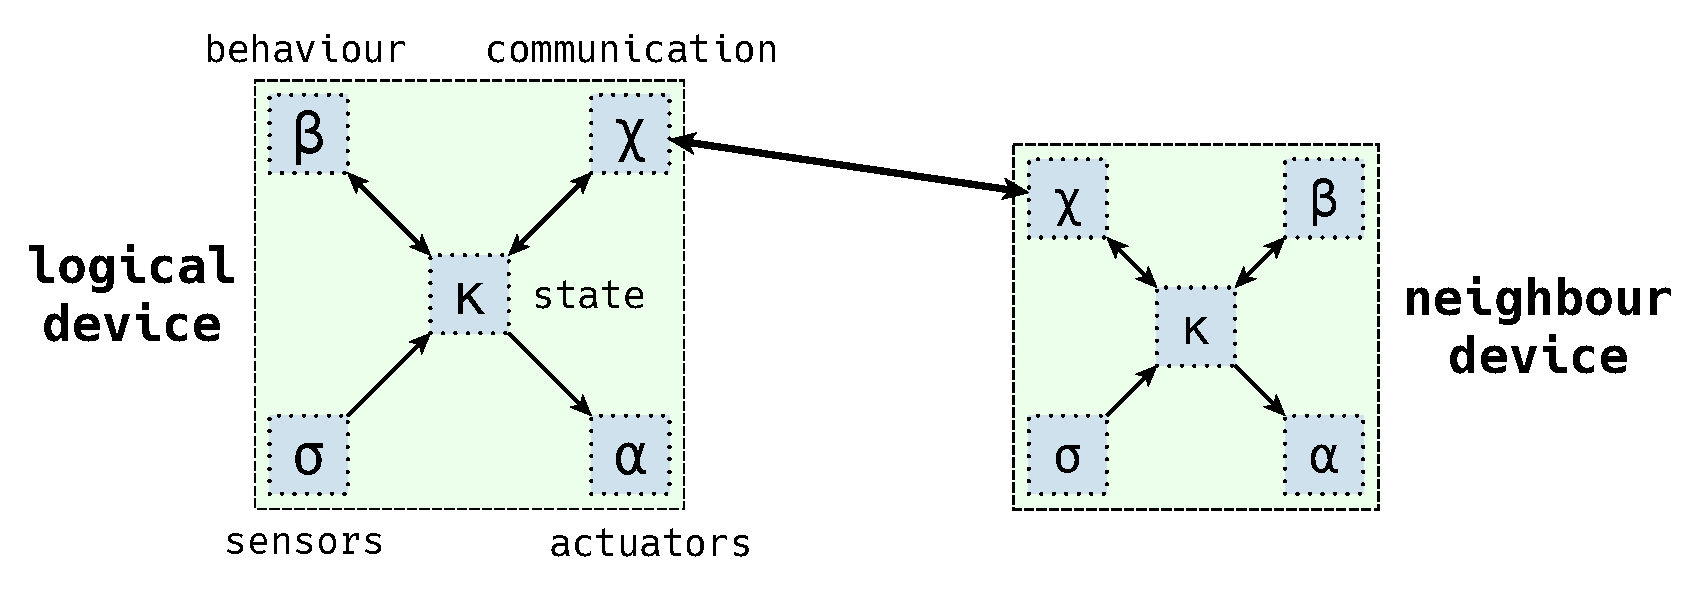
\includegraphics[width=\textwidth]{figures/original-components-interactions.pdf}
	\caption{Representation of a logical device split into its components and a connection with one of its neighbours}
	\label{fig:logical-device}
\end{figure}

Henceforth, concepts characterizing pulverization will be used with the meaning given in~\Cref{tab:ubiquitous-language}.

A \emph{Logical Device} is the representation of a device in the system abstracting from the specific deployment details.
It is composed of \emph{five} components: \emph{Sensors}, \emph{Actuators}, \emph{Behaviour}, \emph{Communication} and \emph{State} while the
interaction between them determines the device's logic in the system. The~\Cref{fig:logical-device} shows a representation of a logical device
split into its components defining also a link with another device.

The \emph{Sensors} $\sigma$ and \emph{Actuators} $\alpha$ components represent the way the device interacts with the environment: the former is used
to acquire information from the environment, while the latter is used to perform actions on the environment.
The \emph{State} $\kappa$ component represents the device's knowledge and abstract from the actual storage mechanism or representation.
The \emph{Communication} $\chi$ component handles the interaction with neighbours by holding the information about the identity of the neighbours and
how to reach them. The send and receive operations occur through respectively the \emph{input channels} and the \emph{output channels}, where the
output channel of a device is connected to the input channel of its neighbours.
Finally, the \emph{Behaviour} $\beta$ component models the device behaviour via a \emph{function} which maps the state of the device to a new state,
defines a set of prescriptive actions to be performed and a set of coordination data to be propagated to the neighbours.

Each device performs a MAPE-like cycle that includes the following steps and that defines the interactions between the device's subcomponents as
depicted in~\Cref{fig:logical-device}, where the arrows denote the message flow:

\begin{enumerate}
	\item \textbf{Context acquisition:} the device acquires information from its sensors and the communication component, storing them in the device
	      state
	\item \textbf{Computation:} the device behaviour function is computed against the device state
	\item \textbf{Coordination data propagation:} coordination data is sent to all the neighbour's device
	\item \textbf{Actuation:} the actuators are activated to execute a set of prescriptive actions
\end{enumerate}

A platform is a collection of physical \emph{hosts} connected by a dynamic graph of physical network links, representing the communication channel
between two hosts. A host is an entity with a unique identifier (e.g. an IP address, URI resource, etc.) and can be a computer system, an embedded
device holding sensors and actuators, a virtual machine or a software container. The type of communication channel (the link between hosts) may
vary depending on the underlying network infrastructure and protocols.
The \emph{hosts} types are divided into two categories: \emph{thin hosts} and \emph{thick hosts}. Thin hosts are devices with limited computational
power and memory, while thick hosts can compute and may even do so on behalf of multiple logical devices.

\begin{figure}
	\centering
	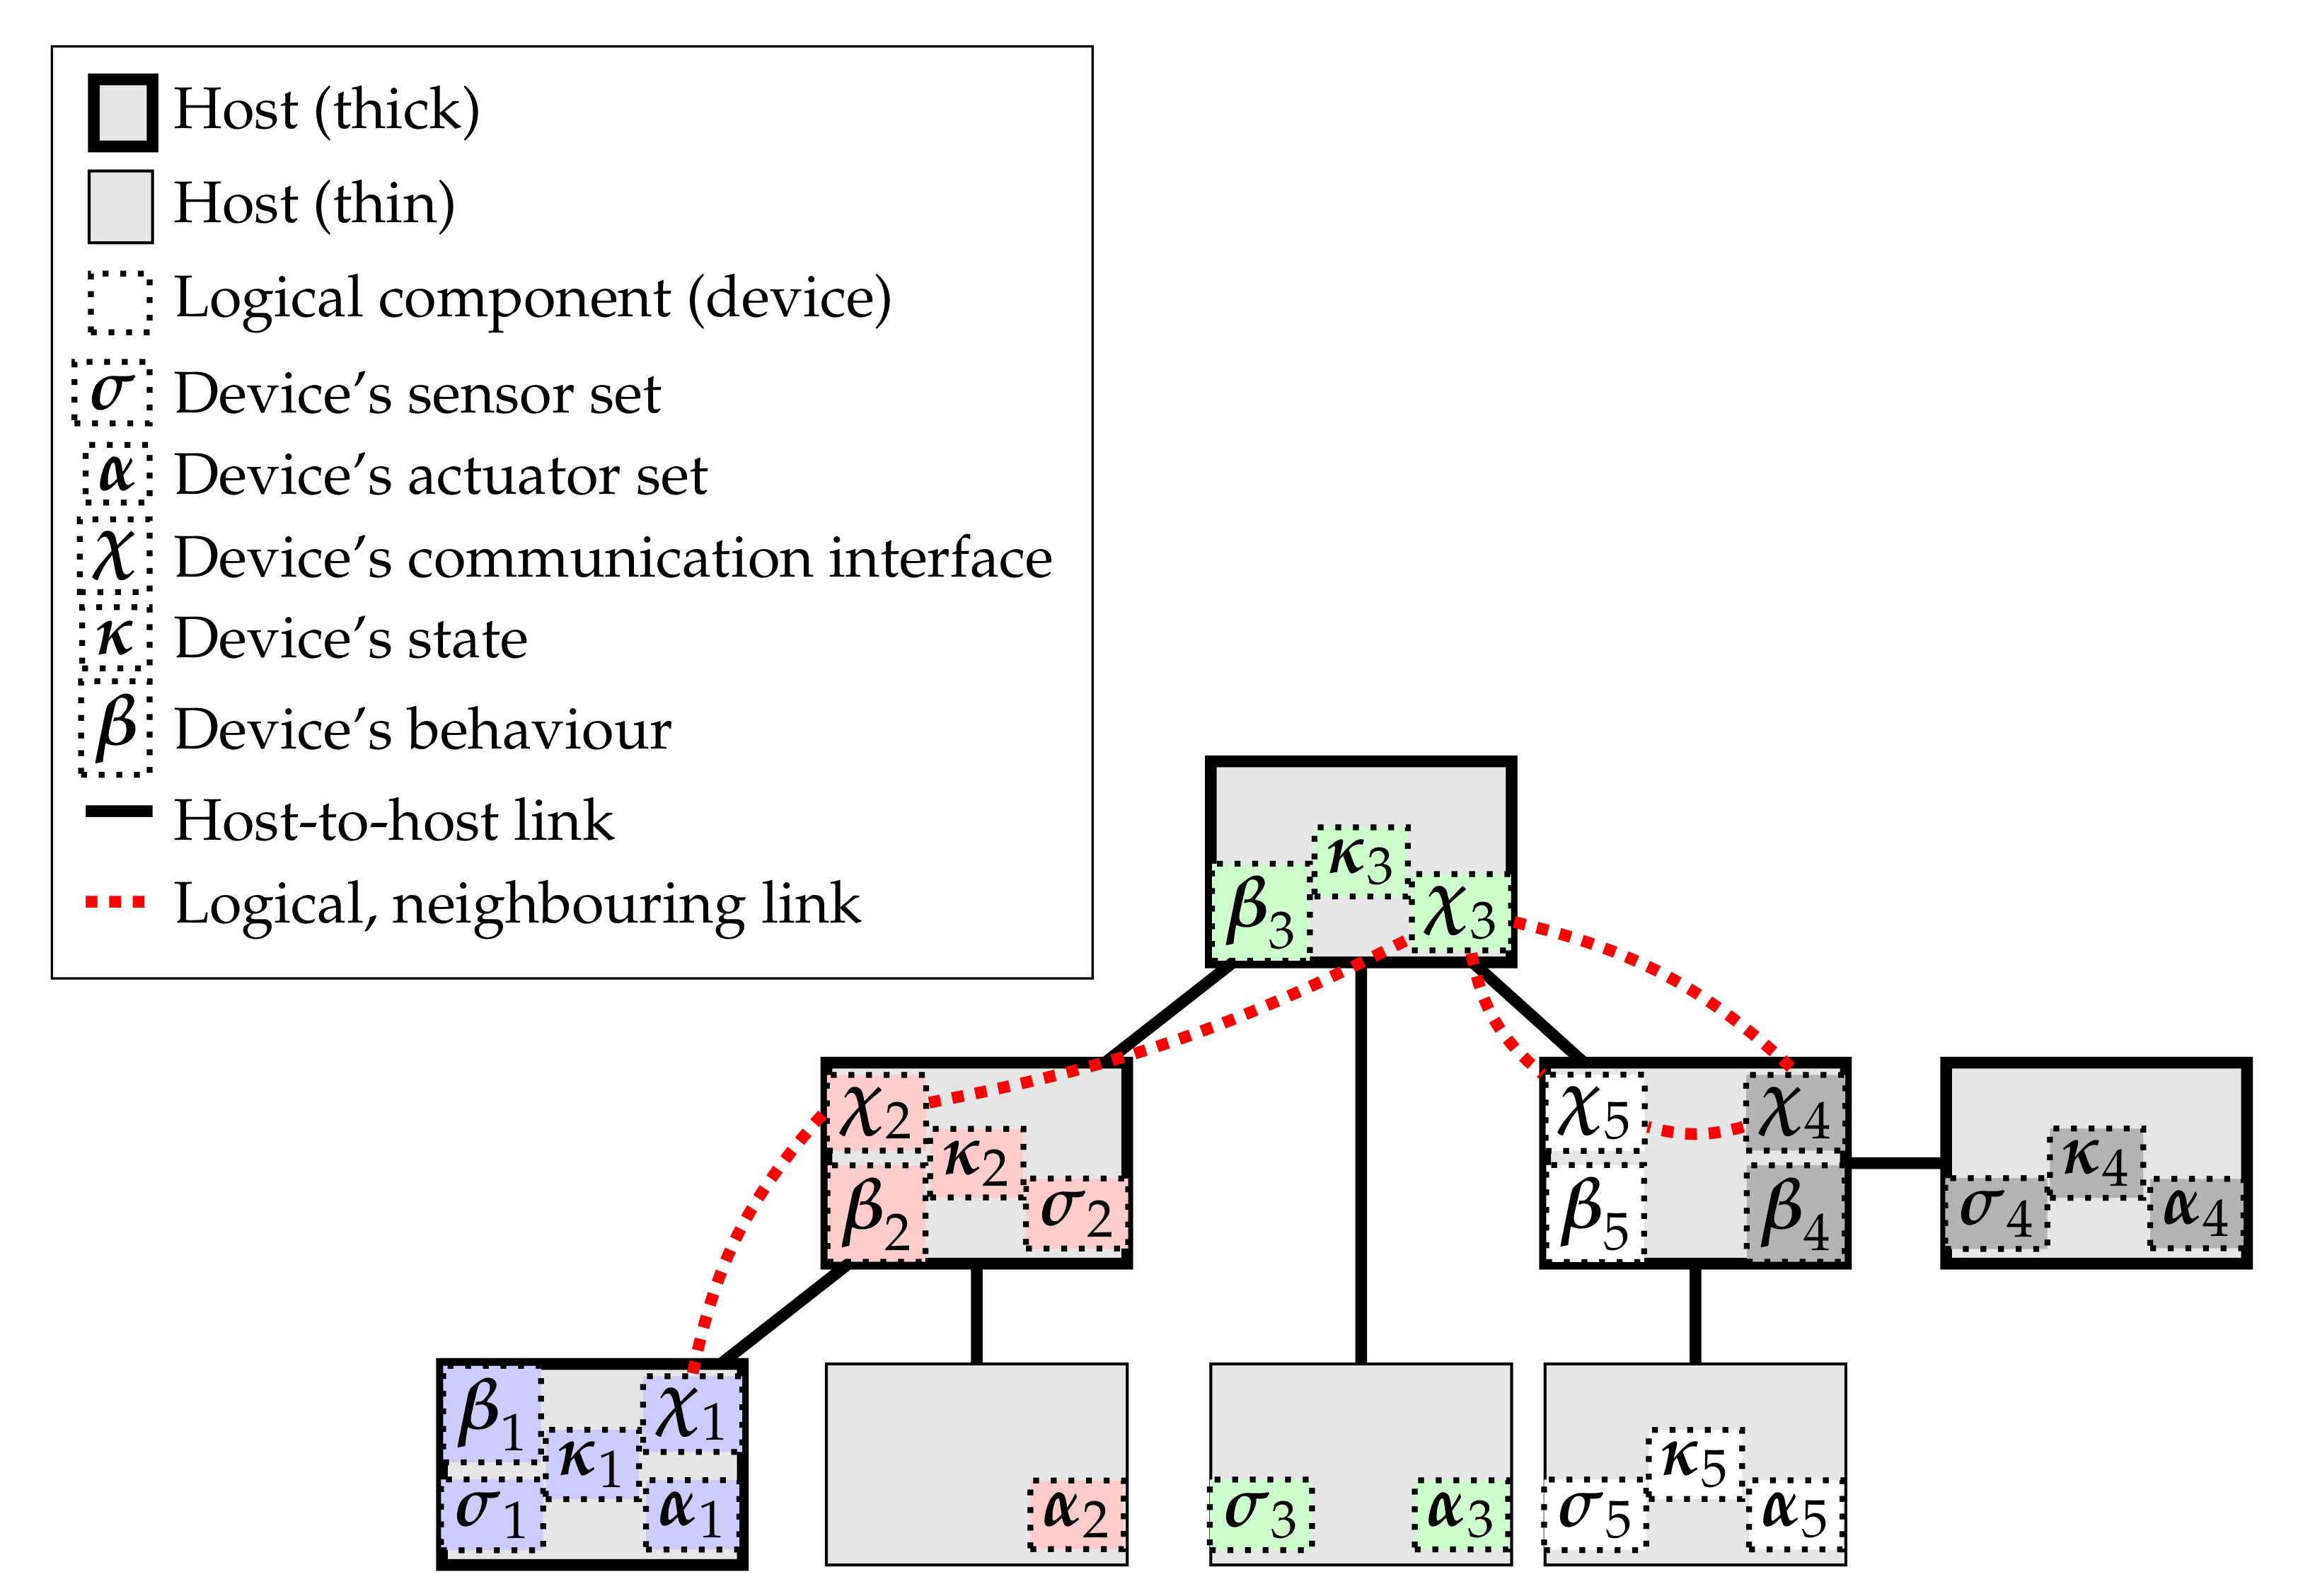
\includegraphics[width=0.7\linewidth]{figures/cps-example.png}
	\caption{Example of instantiation of the CPS model. Picture taken from~\cite{fi12110203}.}
	\label{fig:cps-example}
\end{figure}

\begin{figure}
	\centering
	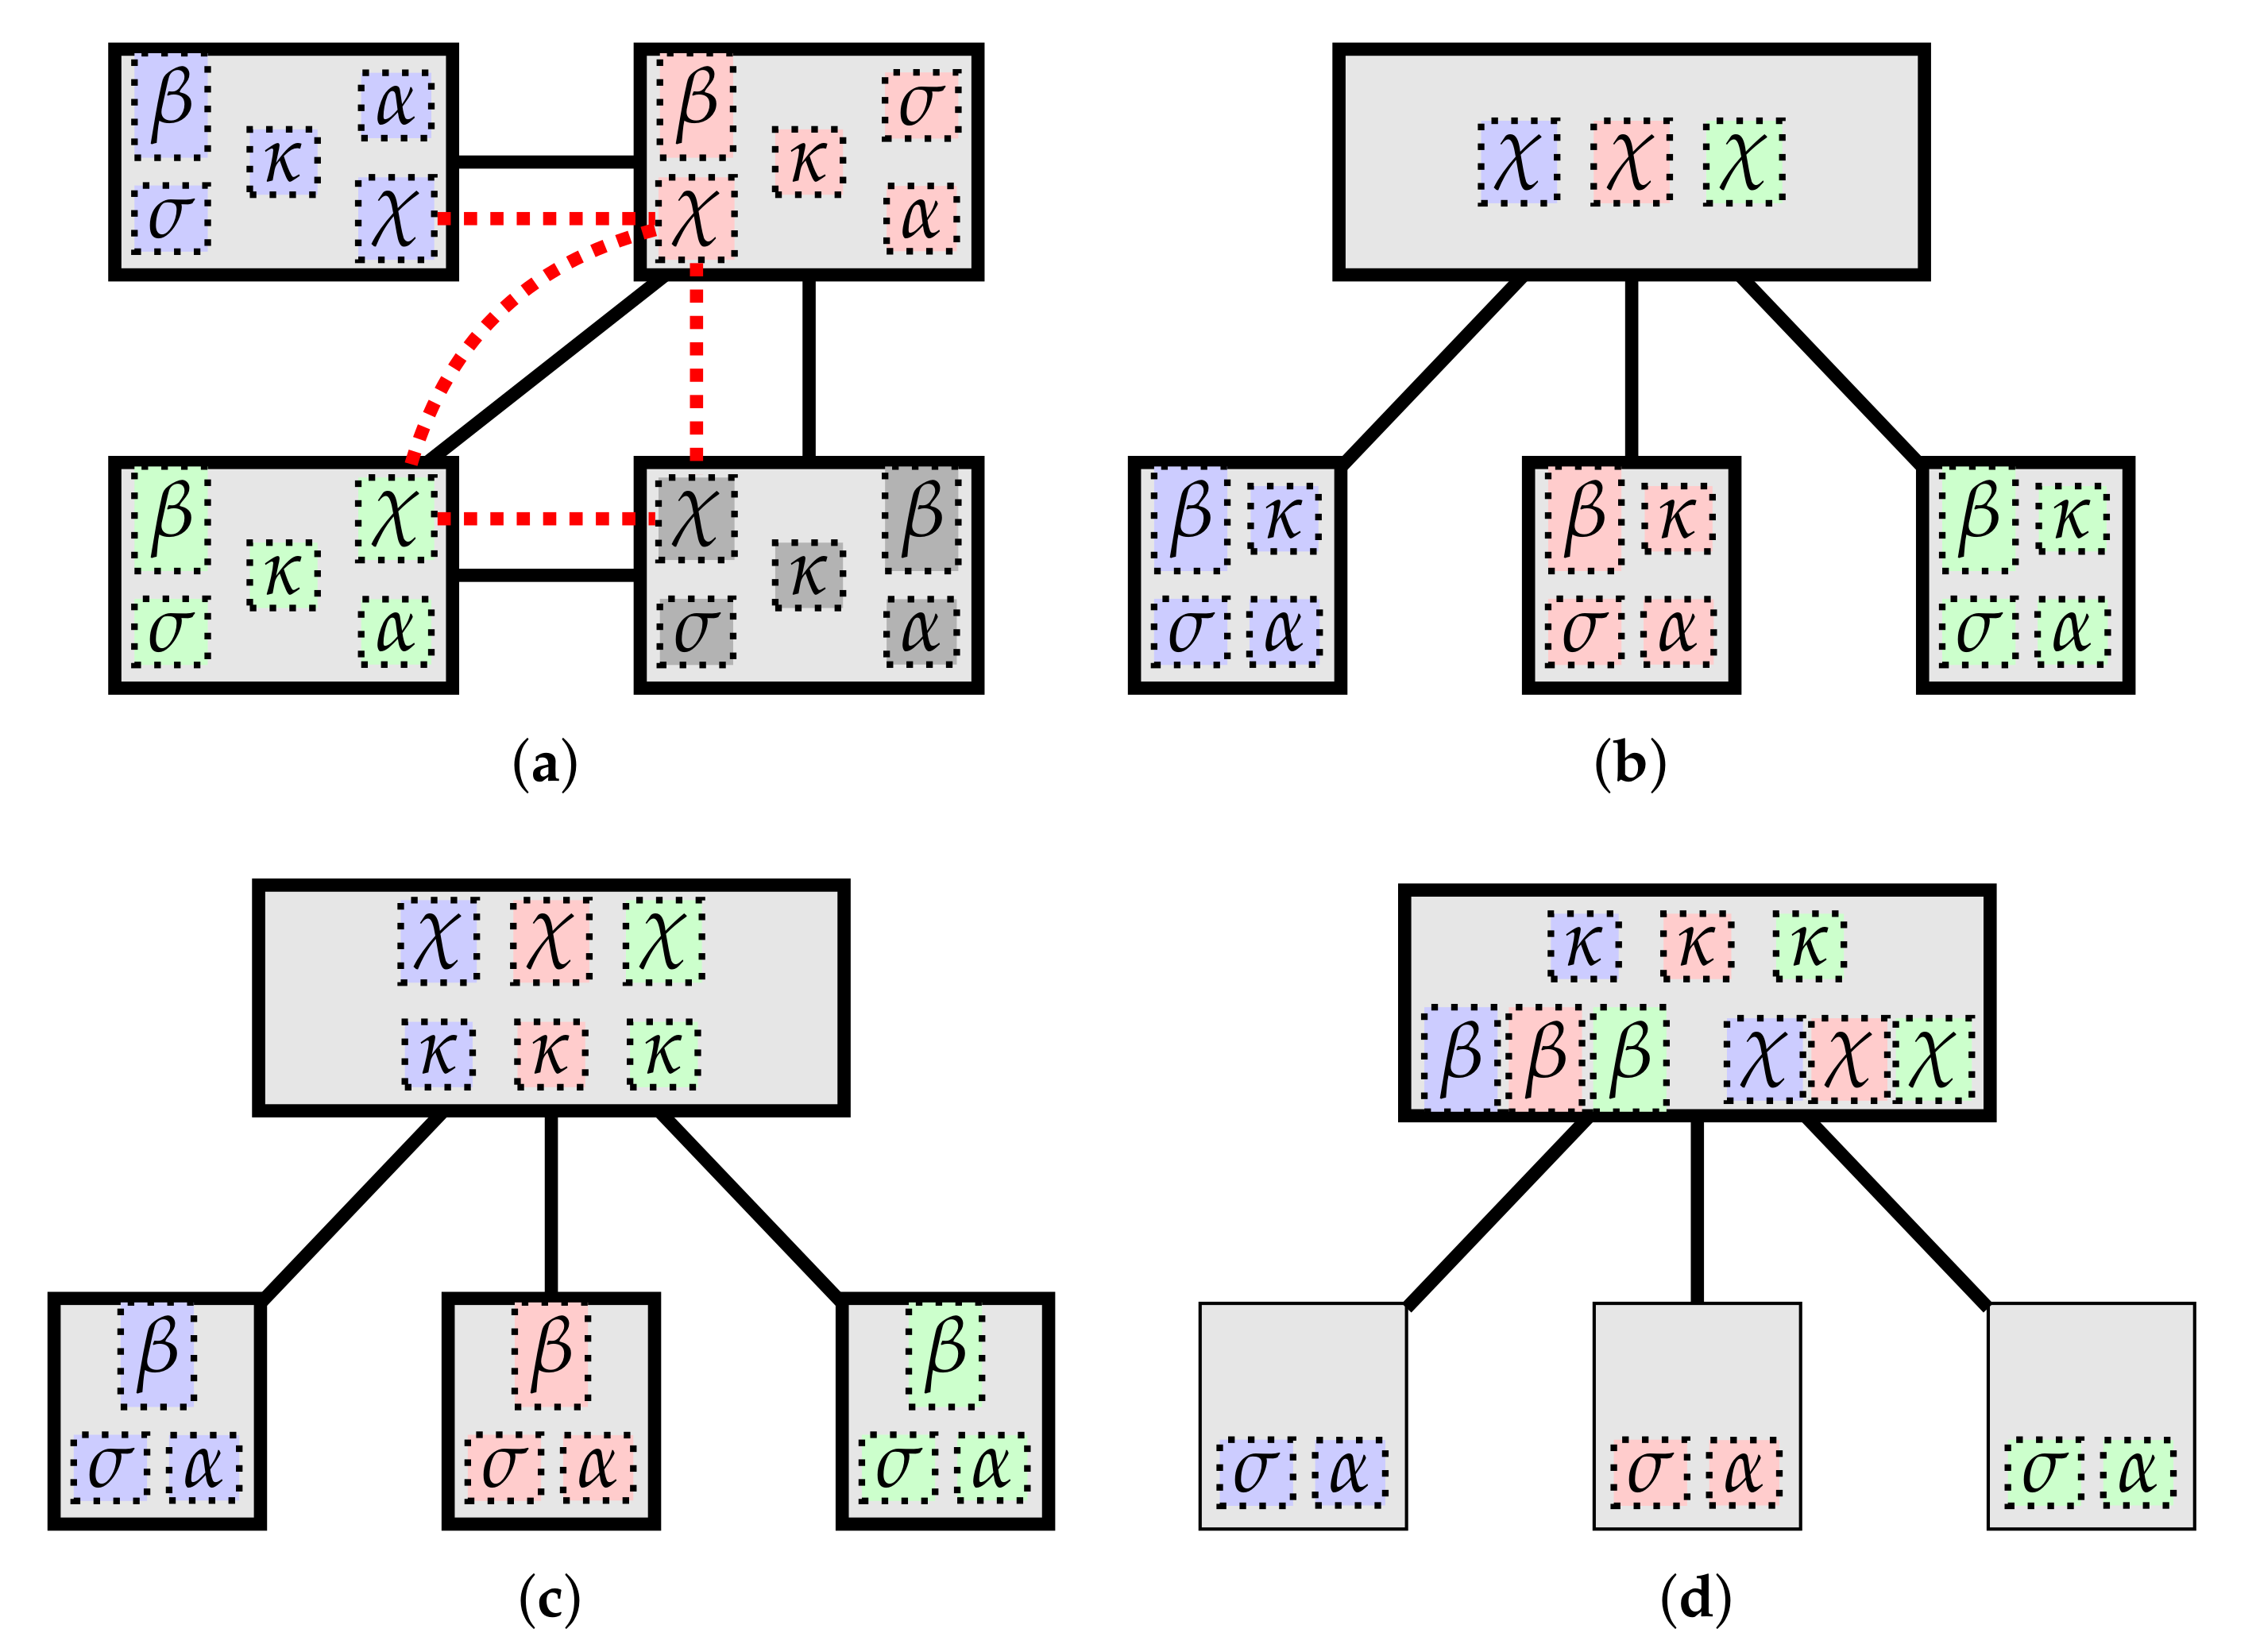
\includegraphics[width=0.7\linewidth]{figures/notable-deployments.png}
	\caption{\textbf{(a)} Peer-to-peer style; \textbf{(b)} broker-based style (e.g. MQTT); \textbf{(c)} Big data in the cloud style; \textbf{(d)} embedded device with sensors/actuators. Picture taken from~\cite{fi12110203}.}
	\label{fig:notable-deployments}
\end{figure}

The deployment of the CPS can be defined as an \emph{allocation map} placing each component of each device to specific hosts in the platform.
An example of a deployment can be seen in~\Cref{fig:cps-example}. In the example is assumed that all the sensors and actuators are deployed on the
same host, though this is not a requirement, sensors and actuators may be deployed on different hosts.

Examples of deployment are provided in~\Cref{fig:notable-deployments} showing an increasing number of responsibilities are centralized.
The~\Cref{fig:notable-deployments}a shows a peer-to-peer style deployment where, for each device, all the components are deployed on the same host.
This style is not suitable in a sensor network where a device is designed to operate for a long time using solely battery power and is not equipped
with enough power to host a $\beta$-component.
The~\Cref{fig:notable-deployments}b shows a broker-based style deployment where all the $\chi$-components are deployed on a separate host (broker).
This is a common scenario in IoT systems where a broker is used to handle the communication between devices.
The~\Cref{fig:notable-deployments}c shows ``big data in the cloud'' style deployment where all the $\kappa$-components are deployed in the cloud
enabling big-data analysis.
The~\Cref{fig:notable-deployments}d shows an embedded device with sensors/actuators style deployment where all the $\alpha$ and $\sigma$-components
are deployed on the same thin host while all the remaining components are deployed on a thick host. This scenario covers the case of a device
with limited computational power and memory by offloading the $\beta$-component to a thick host.

% - New section ---------------------------------------------------------------

\section{Framework requirements}
\label{sec:framework-requirements}

The main objective of this thesis work is to develop a framework that can ``fill the gap'' between the modelling of a CPS (and its simulation) and
the physical deployment of the system on an infrastructure.
The framework should model the pulverization concept and provide a clear separation between the behaviour of the overall system and low-level
details of the deployment via a simple and concise API.
Also, the framework must capture the concepts defined by the pulverizing approach to provide a good starting point on which the framework can
be evolved.

\subsubsection{Business requirements}
\label{sec:business-requirements}

As previously mentioned, the main objective of the framework is to provide a way to deploy CPSs via the pulverization approach.
The business requirements identified are reported as follows:

\begin{itemize}
	\item The pulverization approach can be used to simply and effectively deploy CPS systems
	\item The framework should be flexible to support different deployment strategies
	\item The framework should be extensible to support different communication protocols
\end{itemize}

\subsubsection{User requirements}
\label{sec:user-requirements}

The user requirements are identified from the perspective of the developer who will use the framework.
The user requirements identified are reported as follows:

\begin{itemize}
	\item It should be possible to configure the system to deploy by defining the structure of each device \emph{logical device}
	\item It should be possible to configure the \emph{deployment unit} for each \emph{logical device}
	\item It should be possible to configure the \emph{logical devices} and \emph{deployment unit} via a DSL
	\item It should be possible to create a \emph{sensors} component
	\item It should be possible to create a \emph{actuators} component
	\item It should be possible to create a \emph{communication} component
	\item It should be possible to create a \emph{behaviour} component
	\item It should be possible to create a \emph{state} component
\end{itemize}

\subsubsection{Functional requirements}
\label{sec:functional-requirements}

The functional requirements, obtained from the user requirements, are reported below:

\begin{itemize}
	\item Multiple \emph{logical devices} can be defined
	\item For each \emph{logical device}, the \emph{components} that compose it can be defined
	\item Each \emph{component} defined for a \emph{logical device} must be configured to be deployed on a specific tier of the infrastructure
	\item A check must be performed to ensure that the configuration of the \emph{logical devices} is valid and consistent
	\item Links between \emph{logical devices} can be defined
	\item Multiple deployment units can be defined for each \emph{logical device} using the system configuration
	\item The user-defined \emph{components} can be added to the deployment unit
	\item The \emph{deployment unit} can be started
	\item The \emph{deployment unit} can be stopped
	\item Prevent the run of the \emph{deployment unit} if the configuration is not honored
	\item Different protocols can be added to the \emph{deployment unit} to enable intra-component communication
	\item For each component, a custom implementation of the logic that implements how the communication with other components should occur can be
	      provided
\end{itemize}

\subsubsection{Non-functional requirements}
\label{sec:non-functional-requirements}

\begin{itemize}
	\item The framework should be easy to use by providing a simple and clean API simplifying the development of the system and adoption of the
	      framework
	\item The framework should be extensible in the sense that the user can customize some aspects of the framework like the communication protocols,
	      and the logic of each component
	\item The framework should be flexible to support different deployment strategies coping with different scenarios and infrastructures
	\item The framework should support a wide range of architectures to support a heterogeneous set of devices enabling wide adoption of the
	      framework
\end{itemize}

% - New section ---------------------------------------------------------------

\section{Reference scenarios}
\label{sec:reference-scenarios}

This section gives examples of scenarios in which the framework can be used to implement a Cyber-Physical System.
The proposed scenarios are intended on the one hand to show in what contexts the framework can operate and on the other hand to provide guiding
examples of using the framework for users interested in using it.

The following are three examples that can be used as a reference for applying the pulverization approach.

The first example is the simplest scenario where the pulverization can fit in and can be considered the ``hello world'' of the pulverization.
The scenario is a simple system composed of a single \emph{device} whose objective is to control the moisture level of the soil.
The \emph{device} is composed of a sensor that measures the moisture level of the soil and an actuator that controls the irrigation system.
The objective is to keep the moisture level of the soil at a predefined level. From this description emerge a device composed of the following
components: \emph{sensor, actuator, behaviour,} and \emph{state}. The system is deployed on three hosts: two \emph{thin host} which host the
\emph{sensor} and \emph{actuator} components and a \emph{thick host} which hosts the \emph{behaviour} and \emph{state} components.
In this scenario, the device is ``decomposed'' into sub-component that are deployed on different hosts and the communication between the
components is handled by the framework obtaining the global behaviour of the device. This example shows the basic building blocks of pulverization
by realizing a system with only one device focusing on the use of either \emph{thin hosts} and \emph{thick hosts.}

The second example is a more complex scenario where multiple devices come into play and where communication between them is the main focus.
In this example, two types of devices are defined: one that needs to find another device and the device that needs to be found.
The first device described may be a smartphone, while the second may be an embedded device with low computational and memory characteristics.
The goal of this example is to use smartphones to find the embedded device: the closer the smartphones get to the embedded device, the more intense
light the embedded device will produce; conversely, as the smartphones move away, the light will decrease in intensity.
Meanwhile, smartphones communicate with each other by exchanging information about the distance to the embedded device that needs to be found.
On smartphones are executed the \emph{sensor} and \emph{actuator} components, while \emph{behavior} and \emph{state} components are offloaded to the
cloud. Similarly, the embedded device hosts only the \emph{actuator} component while the \emph{behavior} is offloaded to the cloud. As for 
communication between the devices, all \emph{communication} components are instantiated in the cloud.
This scenario emphasizes the communication that takes place between devices in the system: devices are decomposed into their components that are then
instantiated in the infrastructure where communication does not reside in the devices themselves but rather on the cloud, nevertheless the
correctness of system operation will be preserved.

The last example proposed is quite similar to the previous one but the focus is on having some devices perform the behavior locally while others 
are offloaded to the cloud. This example is intended to show that it is possible to support different ways of deploying the system seamlessly.
The goal of the example is to implement a system that measures the level of aggregation of people (leveraging a mobile device) through, for example,
a crowd estimation algorithm.
The system consists of many devices that interact with each other and exchange information about the distance between them. This information is then
shared with an additional device in the network that is responsible for making an estimate of the crowd and performing an actuation proportional
to the computed value. The peculiarity of this deployment lies in the fact that some devices perform the behavior computation on the device itself, 
while other devices perform the computation offloaded in the cloud. Thus, by varying the system deployment strategy for the same device, we want to 
observe that the system maintains its functional correctness.
